%%%%%%%%%%%%%%%%%%%%%%%%%%%%%%%%%%%%%%%%%%%%%%%%%%%%%%%%%%%%%%%%
%%%%%%%%%%%%%%%%%%%%%%%%%%%%%%%%%%%%%%%%%%%%%%%%%%%%%%%%%%%%%%%%
%%%%
%%%% This text file is part of the source of 
%%%% `Introduction to High-Performance Scientific Computing'
%%%% by Victor Eijkhout, copyright 2012
%%%%
%%%% This book is distributed under a Creative Commons Attribution 3.0
%%%% Unported (CC BY 3.0) license and made possible by funding from
%%%% The Saylor Foundation \url{http://www.saylor.org}.
%%%%
%%%%
%%%%%%%%%%%%%%%%%%%%%%%%%%%%%%%%%%%%%%%%%%%%%%%%%%%%%%%%%%%%%%%%
%%%%%%%%%%%%%%%%%%%%%%%%%%%%%%%%%%%%%%%%%%%%%%%%%%%%%%%%%%%%%%%%

\Level 1 {Theory of general iterative methods}
\label{sec:nonstationary}

Above, you saw iterative methods of the form $x_{i+1}=x_i-K\inv r_i$,
and we will now see iterative methods of the more general form
\begin{equation}
  x_{i+1}=x_i+\sum_{j\leq i}K\inv r_j\alpha_{ji},
  \label{eq:it-general-x}
\end{equation}
that is, using all previous residuals to update the iterate.
One might ask, `why not introduce an extra
parameter and write $x_{i+1}=\alpha_i x_i+\cdots$?' Here we give a
short argument that the former scheme describes a large class of
methods. Indeed, the current author is not aware of methods that fall
outside this scheme.

We defined the residual, given an approximate solution~$\tilde x$, as
$ \tilde r=A\tilde x-b $. For this general discussion we precondition the system
as $K\inv Ax=K\inv b$. (See section~\ref{sec:preconditioner} where we
discussed transforming the linear system.)
The corresponding residual for the initial
guess~$\tilde x$ is
\[ \tilde r = K\inv A\tilde x-K\inv b. \]
We now find that 
\[ x=A\inv b=\tilde x-A\inv K\tilde r = \tilde x-(K\inv A)\inv \tilde r. \]
%
Now, the \indexterm{Cayley-Hamilton theorem} states that for
every~$ A $ there exists a polynomial~$\phi(x)$ (the
\indexterm{characteristic polynomial}) such that
\[ \phi(A)=\nobreak0 .\]
We observe that we can write this polynomial $\phi$ as
\[ \phi(x)=1+x\pi(x) \]
where $\pi$ is another polynomial.
%
Applying this to $K\inv A$, we have
\[
  0 = \phi( K\inv A ) = I + K\inv A \pi( K\inv A ) 
  \Rightarrow
  (K\inv A)\inv=-\pi(K\inv A)
\]
so that $ x = \tilde x + \pi(K\inv A)\tilde r $. Now, if we let
$x_0=\tilde x$, then $\tilde r = K\inv r_0$, giving the equation
\[ x = x_0 + \pi(K\inv A)K\inv r_0. \]

This equation suggests an iterative scheme: if we can find a
series of polynomials~$\pi^{(i)}$ of degree~$i$
to approximate~$\pi$, it will give
us a sequence of iterates 
\begin{equation}
  x_{i+1} = x_0+\pi^{(i)}(K\inv A)K\inv r_0
  = x_0+K\inv \pi^{(i)}(AK\inv) r_0
  \label{eq:x-from-PA-r0}
\end{equation}
that ultimately reaches the true solution.
Multiplying this equation by~$A$ and subtracting~$b$ on both sides gives
\[ r_{i+1} = r_0+\tilde\pi^{(i)}(AK\inv)r_0 \]
where $\tilde\pi^{(i)}(x)=x\pi^{(i)}(x)$. This immediately gives us
\begin{equation}
  r_i = \hat\pi^{(i)}(AK\inv) r_0
  \label{eq:r-is-polynomial}
\end{equation}
where $\hat\pi^{(i)}$ is a polynomial of degree~$i$ with
$\hat\pi^{(i)}(0)=\nobreak1$. This statement can be used as the basis
of a convergence theory of iterative methods. However, this goes
beyond the scope of this book.

Let us look at a couple of instances of
equation~\eqref{eq:r-is-polynomial}. For $i=1$ we have
\[
  r_1 = (\alpha_1AK\inv+\alpha_2I)r_0 \Rightarrow 
  AK\inv r_0 = \beta_1r_1+\beta_0r_0
\]
for some values $\alpha_i,\beta_i$. For $i=2$
\[ r_2 = (\alpha_2(AK\inv )^2+\alpha_1AK\inv +\alpha_0)r_0 \]
for different values~$\alpha_i$. But we had already established that
$AK\inv_0$ is a combination of $r_1,r_0$, so now we have that 
\[ (AK\inv)^2r_0\in \setspan{r_2,r_1,r_0}, \]
and it is clear how to show inductively that 
\begin{equation}
  (AK\inv)^ir_0\in\setspan{r_i,\ldots,r_0}.
\end{equation}
Substituting this in \eqref{eq:x-from-PA-r0} we finally get
\begin{equation}
  x_{i+1} = x_0 +\sum_{j\leq i} K\inv r_j\alpha_{ji}.
  \label{eq:iterate-general-x0}
\end{equation}
It is easy to see that the scheme \eqref{eq:it-general-x} is of the
form~\eqref{eq:iterate-general-x0} and
that the reverse implication also holds.

Summarizing, the basis of iterative methods is a scheme where
iterates get updated by all residuals computed so far:
\begin{equation}
  x_{i+1} = x_i+\sum_{j\leq i}K\inv r_j\alpha_{ji}.
  \label{eq:preconditioned-iteration}
\end{equation}
Compare that to the stationary iteration
(section~\ref{sec:stationary}) where the iterates get updated from
just the last residual, and with a coefficient that stays constant.

We can say more about the $\alpha_{ij}$ coefficients.
If we multiply equation~\eqref{eq:preconditioned-iteration} by~$A$,
and subtract $b$ from both sides,
we find
\begin{equation}
  r_{i+1} = r_i+\sum_{j\leq i}AK\inv r_j\alpha_{ji}.
  \label{eq:general-r-update}
\end{equation}
Let us consider this equation for a moment. If we have a starting
residual~$r_0$, the next residual is computed as
\[ r_1=r_0+AK\inv r_0\alpha_{00}. \]
From this we get that $AK\inv r_0 = \alpha_{00}\inv(r_1-r_0)$, so
for the next residual,
\[
\begin{array}{rl}
  r_2&=r_1+AK\inv r_1\alpha_{11}+AK\inv r_0\alpha_{01}\\
  &=r_1+AK\inv r_1\alpha_{11}+\alpha_{00}\inv\alpha_{01}(r_1-r_0)\\
  \Rightarrow AK\inv r_1&=\alpha_{11}\inv
  (r_2-(1+\alpha_{00}\inv\alpha_{01})r_1+\alpha_{00}\inv\alpha_{01}r_0)
\end{array}
\]
We see that we can express $AK\inv r_1$ as a sum
$r_2\beta_2+r_1\beta_1+r_0\beta_0$, and that $\sum_i\beta_i=0$. 

Generalizing this, we find (with different $\alpha_{ij}$ than above)
\[ 
\begin{array}{rll}
  r_{i+1}&=r_i+AK\inv r_i\delta_i+\sum_{j\leq i+1}r_j\alpha_{ji}\\
  r_{i+1}(1-\alpha_{i+1,i})&=AK\inv r_i\delta_i +r_i(1+\alpha_{ii})
      +\sum_{j< i} r_j\alpha_{ji}\\
  r_{i+1}\alpha_{i+1,i}&=AK\inv r_i\delta_i +
      \sum_{j\leq i}r_j\alpha_{ji}
      &\vtop{
        \hbox{substituting $\begin{array}{ll}\alpha_{ii}:=1+\alpha_{ii}\\
        \alpha_{i+1,i}:=1-\alpha_{i+1,i}\end{array}$}
        \hbox{note that $\alpha_{i+1,i}=\sum_{j\leq i}\alpha_{ji}$}
        }\\
  r_{i+1}\alpha_{i+1,i}\delta_i\inv&=AK\inv r_i +\sum_{j\leq i}
  r_j\alpha_{ji}\delta_i\inv\\  
  r_{i+1}\alpha_{i+1,i}\delta_i\inv&=AK\inv r_i +\sum_{j\leq i}
      r_j\alpha_{ji}\delta_i\inv\\
  r_{i+1}\gamma_{i+1,i}&AK\inv r_i+\sum_{j\leq i} r_j\gamma_{ji}
      &\hbox{substituting $\gamma_{ij}=\alpha_{ij}\delta_j\inv$}
\end{array}
\]
and we have that $\gamma_{i+1,i}=\sum_{j\leq i}\gamma_{ji}$.

We can take this last equation and write it as $AK\inv R=RH$ where
\[ H=
\begin{pmatrix}
  -\gamma_{11}&-\gamma_{12}&\ldots\\
  \gamma_{21}&-\gamma_{22}&-\gamma_{23}&\ldots\\
  0&\gamma_{32}&-\gamma_{33}&-\gamma_{34}\\
  \emptyset&\ddots&\ddots&\ddots&\ddots
\end{pmatrix}
\]
In this, $H$~is a so-called \indexterm{Hessenberg matrix}: it is upper
triangular plus a single lower subdiagonal. Also we note that the
elements of~$H$ in each column sum to zero.

Because of the identity $\gamma_{i+1,i}=\sum_{j\leq i}\gamma_{ji}$ we
can subtract~$b$ from both sides of the equation for~$r_{i+1}$ and
`divide out~$A$', giving
\[
  x_{i+1}\gamma_{i+1,i}=K\inv r_i+\sum_{j\leq i} x_j\gamma_{ji}.
\]
This gives us the general form for iterative methods:
\begin{equation}
  \begin{cases}
    r_i = Ax_i-b\\
    x_{i+1}\gamma_{i+1,i}=K\inv r_i+\sum_{j\leq i} x_j\gamma_{ji}\\
    r_{i+1}\gamma_{i+1,i}=AK\inv r_i+\sum_{j\leq i} r_j\gamma_{ji}
  \end{cases}\qquad
  \hbox{where $\gamma_{i+1,i}=\sum_{j\leq i}\gamma_{ji}$}.
  \label{eq:general-xr-hessenberg}
\end{equation}
This form holds for many iterative methods, including the stationary
iterative methods you have seen above. In the next sections you will
see how the $\gamma_{ij}$ coefficients follow from orthogonality
conditions on the residuals.

\Level 1 {Iterating by orthogonalization}
\label{sec:fom}

The stationary methods described above (section~\ref{sec:stationary})
have been around in some form or another for a long time: Gauss
described some variant in a letter to a student. They were perfected
in the thesis of Young~\cite{Young:thesis} in 1950; the final
reference is probably the book by
Varga~\cite{Varga:iterative-analysis}. These methods are little used
these days, except in the specialized context of \indexterm{multigrid}
\indexterm{smoothers}, a~topic not discussed in this course.

At almost the same time, the
field of methods based on orthogonalization was kicked off by two
papers~\cite{Lanczos1952:solution_of_systems,HestenesStiefel1952:cg},
though it took a few decades for them to find wide applicability. (For
further history, see~\cite{GolubOleary:cg-history}.)

The basic idea is as follows:
\begin{quote}
  If you can make all your residuals orthogonal to each other, and the
  matrix is of dimension~$n$, then after $n$ iterations you have to
  have converged: it is not possible to have an $n+1$-st residual that
  is orthogonal to all previous and nonzero. Since a zero residual
  means that the corresponding iterate is the solution, we conclude
  that after $n$ iterations we have the true solution in hand.
\end{quote}
With the size of matrices that contemporary applications generate this
reasoning is no longer relevant: it is not computationally realistic
to iterate for $n$ iterations. Moreover, roundoff will probably destroy any
accuracy of the solution.
%
However, it was later realized~\cite{Reid1971:cg} that such methods
\emph{are} a realistic option in the case of \indexacf{SPD} matrices. The
reasoning is then:
\begin{quote}
  The sequence of residuals spans a series of subspaces of increasing
  dimension, and by orthogonalizing, the new residuals are projected on
  these spaces. This means that they will have decreasing sizes.
\end{quote}
\begin{figure}[ht]
  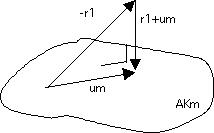
\includegraphics[scale=.7]{graphics-public/projection}
  \caption{The optimal update $u_m$ make the new residual orthogonal to
    the $AK_m$ subspace}
  \label{fig:res-projection}
\end{figure}
This is illustrated in figure~\ref{fig:res-projection}.

In this section you will see the basic idea of iterating by
orthogonalization. The method presented here is only of theoretical
interest; next you will see the \acf{CG} and \acf{GMRES} methods that
are the basis of many real-life applications.

Let us now take the basic scheme \eqref{eq:general-xr-hessenberg} and
orthogonalize the residuals. Instead of the normal inner product we
use the $K\inv$-inner product:
\[ (x,y)_{K\inv} = x^tK\inv y \]
and we will force residuals to be $K\inv$-orthogonal:
\[ \forall_{i\not=j}\colon r_i\perp_{K\inv} r_j \Leftrightarrow
   \forall_{i\not=j}\colon r_iK\inv r_j=0
\]
This is known as the \indexacf{FOM}
scheme:
\begin{quote}
  \begin{tabbing}
    Let $r_0$ be given\\
    For \=$i\geq 0$:\\
    \>let $s\leftarrow K\inv r_i$\\
    \>let $t\leftarrow AK\inv r_i$\\
    \>for \=$j\leq i$:\\
    \>\>let $\gamma_j$ be the coefficient so that $t-\gamma_jr_j\perp r_j$\\
    \>for \=$j\leq i$:\\
    \>\>form \=$s\leftarrow s-\gamma_jx_j$\\
    \>\>and  \>$t\leftarrow t-\gamma_jr_j$\\
    \>let $x_{i+1}=(\sum_j\gamma_j)\inv s$,
    $r_{i+1}=(\sum_j\gamma_j)\inv t$.\\
  \end{tabbing}
\end{quote}
You may recognize the \indexterm{Gram-Schmidt} orthogonalization in
this (see appendix~\ref{app:gram-schmidt} for an explanation): in each
iteration $r_{i+1}$ is initially set to $AK\inv r_i$, and orthogonalized
against $r_j$ with~$j\leq\nobreak i$.

We can
use \indextermsub{modified}{Gram-Schmidt} by rewriting the algorithm
as:
\begin{quote}
  \begin{tabbing}
    Let $r_0$ be given\\
    For \=$i\geq 0$:\\
    \>let $s\leftarrow K\inv r_i$\\
    \>let $t\leftarrow AK\inv r_i$\\
    \>for \=$j\leq i$:\\
    \>\>let $\gamma_j$ be the coefficient so that $t-\gamma_jr_j\perp r_j$\\
    \>\>form \=$s\leftarrow s-\gamma_jx_j$\\
    \>\>and  \>$t\leftarrow t-\gamma_jr_j$\\
    \>let $x_{i+1}=(\sum_j\gamma_j)\inv s$,
    $r_{i+1}=(\sum_j\gamma_j)\inv t$.\\
  \end{tabbing}
\end{quote}
These two version of the \ac{FOM} algorithm are 
equivalent in exact arithmetic, but differ in practical circumstances
in two ways:
\begin{itemize}
\item The modified Gramm-Schmidt method is more numerically stable;
\item The unmodified method allows you to compute all inner products
  simultaneously. We discuss this below in
  section~\ref{sec:iterative-computational}.
\end{itemize}
Even though the \ac{FOM} algorithm is not used in practice, these
computational considerations carry over to the \ac{GMRES} method
below.

\Level 1 {Coupled recurrences form of iterative methods}

Above, you saw the general equation \eqref{eq:general-xr-hessenberg}
for generating iterates and search directions.
This equation is often split as
\begin{itemize}
\item An update of the $x_i$ iterate from a single \indexterm{search
  direction}:
\[ x_{i+1}=x_i-\delta_i p_i, \] and
\item A construction of the search direction from the residuals known
  so far:
  \[ p_i = K\inv r_i+\sum_{j<i}\beta_{ij} K\inv r_j. \]
  It is not hard to see inductively that we can also define
  \[ p_i = K\inv r_i+\sum_{j<i}\gamma_{ji} p_j, \]
  and this last form is the one that is used in practice.
\end{itemize}
The iteration dependent coefficients are typically chosen to let the
residuals satisfy various orthogonality conditions. For instance, one
can choose to let the method be defined by letting the residuals be
orthogonal ($r_i^tr_j=0$ if $i\not=j$), or $A$-orthogonal
($r_i^tAr_j=0$ if $i\not=j$). Many more schemes exist.  Such methods
can converge much faster than stationary iteration, or converge for a
wider range of matrix and preconditioner types. Below we will see two
such methods; their analysis, however, is beyond the scope of this
course.

\Level 1 {The method of Conjugate Gradients}
\label{sec:cg}
\indexacstart{CG|(}

In this section, we will derive the \acf{CG} method, which is a
specific implementation of the \ac{FOM} algorithm. In particular, it
has pleasant computational properties in the case of an \ac{SPD}
matrix~$A$.

The \ac{CG} method takes as its basic form the coupled recurrences
formulation described above, and the
coefficients are defined by demanding that
the sequence of residuals $r_0,r_1,r_2,\ldots$ satisfy
\[ r_i^tK\inv r_j=0\quad\hbox{if $i\not=j$}. \]
We start by deriving the \ac{CG} method for nonsymmetric systems, and
then show how it simplifies in the symmetric case. (The approach here
is taken from~\cite{Eijkhout2010ICCS-krylov}).

The basic equations are
\begin{equation}
  \begin{cases}
    x_{i+1}=x_i-\delta_i p_i \\
    r_{i+1}=r_i-\delta_iA p_i \\
    p_{i+1} = K\inv r_{i+1}+\sum_{j\leq i}\gamma_{ji+1} p_j,
  \end{cases}
  \label{eq:xrp-update}
\end{equation}
where the first and third equation were introduced above, and the
second can be found by multiplying the first by~$A$ (check this!).

We will now derive the coefficients in this method by induction. In
essence, we assume that we have current residual $r_{\mathrm{cur}}$, a
residuals to be computed~$r_{\mathrm{new}}$, and a collection of known
residuals~$R_{\mathrm{old}}$. Rather than using subscripts `old, cur,
new', we use the following convention:
\begin{itemize}
\item $x_1,r_1,p_1$ are the current iterate, residual, and search
  direction. Note that the subscript~1 does not denote the iteration
  number here.
\item $x_2,r_2,p_2$ are the iterate, residual, and search direction
  that we are about to compute. Again, the subscript does not equal
  the iteration number.
\item $X_0,R_0,P_0$ are all previous iterates, residuals, and search
  directions bundled together in a block of vectors.
\end{itemize}
In terms of these quantities, the update equations are then
\begin{equation}
\begin{cases}
  x_2=x_1-\delta_1 p_1 \\
  r_2=r_1-\delta_iA p_1 \\
  p_2 = K\inv r_2+\upsilon_{12}p_1+P_0u_{02}
\end{cases}
\label{eq:cg-updates-xrp}
\end{equation}
where $\delta_1,\upsilon_{12}$ are scalars, and $u_{02}$ is a vector with
length the number of iterations before the current. We now derive
$\delta_1,\upsilon_{12},u_{02}$ from the orthogonality of the residuals. To
be specific, the residuals have to be orthogonal under the $K\inv$
inner product: we want to have
\[
  r_2^tK\inv r_1=0,\qquad r_2^tK\inv R_0=0.
\]
Combining these relations gives us, for instance,
\[
  \left.
  \begin{array}{l}
    r_1^tK\inv r_2=0\\   r_2=r_1-\delta_iAK\inv p_1
  \end{array}
  \right\} \Rightarrow
  \delta_1 = \frac{r_1^tr_1}{r_1^tAK\inv p_1}.
\]
Finding $\upsilon_{12},u_{02}$ is a little harder. For this, we start by
summarizing the relations for the residuals and search directions
in equation \eqref{eq:xrp-update} in block
form as 
\[
  (R_0,r_1,r_2) \left(
\begin{array}{r|c|c}
  \begin{matrix}1\\ -1&1\\ &\ddots&\ddots \end{matrix}
  &&\\ \hline -1&1&\\ \hline &-1&1
\end{array}
  \right) = A(P_0,p_1,p_2)\diag(D_0,d_1,d_2)
\]
\[ (P_0,p_1,p_2)
\begin{pmatrix}
  I-U_{00}&-u_{01}&-u_{02}\\ &1&-\upsilon_{12}\\ &&1
\end{pmatrix}
= K\inv (R_0,r_1,r_2)
\]
or abbreviated $RJ=APD$, $P(I-U)=R$ where $J$ is the matrix with
identity diagonal and minus identity subdiagonal. We then observe that
\begin{itemize}
\item $R^tK\inv R$ is diagonal, expressing the orthogonality of the
  residuals.
\item Combining that $R^tK\inv R$ is diagonal and $P(I-U)=R$ gives that
  $R^tP=R^tK\inv R(I-U)\inv$. We now reason that $(I-U)\inv$ is upper
  diagonal, so $R^tP$ is upper triangular. This tells us quantities
  such as $r_2^tp_1$ are zero.
\item Combining the relations for $R$ and~$P$, we get first that
  \[ R^tK\invt AP = R^tK\invt RJD\inv \]
  which tells us that $R^tK\invt AP$ is lower bidiagonal. Expanding $R$ in
  this equation gives
  \[ P^tAP = (I-U)\invt R^tR JD\inv.\]
  Here $D$ and $R^tK\inv R$ are diagonal, and $(I-U)\invt$ and $J$ are lower
  triangular, so $P^tAP$ is lower triangular.
\item This tells us that $P_0^tAp_2=0$ and $p_1^tAp_2=0$.
\item Taking the product of $P_0^tA$, $p_1^tA$ with the definition of
  $p_2$ in equation~\eqref{eq:cg-updates-xrp} gives
  \[ 
     u_{02} = -(P_0^tAP_0)\inv P_0^tAK\inv r_2, \qquad
     \upsilon_{12} = -(p_1^tAp_1)\inv p_1^tAK\inv r_2.
  \]
\item If $A$ is symmetric, $P^tAP$ is lower triangular (see above) and
  symmetric, so it is in fact diagonal. Also, $R^tK\invt AP$ is lower
  bidiagonal, so, using $A=A^t$, $P^tAK\inv R$ is upper bidiagonal. Since
  $P^tAK\inv R=P^tAP(I-U)$, we conclude that $I-U$ is upper bidiagonal, so,
  only in the symmetric case,~$u_{02}=\nobreak 0$.
\end{itemize}

Some observations about this derivation.
\begin{itemize}
\item Strictly speaking we are only proving necessary
  relations here. It can be shown that these are sufficient too.
\item There are different formulas that wind up computing the same
  vectors, in exact arithmetic. For instance, it is easy to derive
  that $p_1^tr_1=r_1^tr_1$, so this can be substituted in the formulas
  just derived. The implementation of the \ac{CG} method as it is
  typically implemented, is given in figure~\ref{fig:pcg}.
\item In the $k$-th iteration, computing $P_0^tAr_2$ (which is needed
  for~$u_{02}$) takes $k$ inner products. First of all, inner products
  are disadvantageous in a parallel context. Secondly, this requires
  us to store all search directions indefinitely. This second point
  implies that both work
  and storage go up with the number of iterations. Contrast this with
  the stationary iteration scheme, where storage was limited to the
  matrix and a few vectors, and work in each iteration was the same.
\item The objections just raised disappear in the symmetric
  case. Since $u_{02}$ is zero, the dependence on $P_0$ disappears,
  and only the dependence on $p_1$ remains. Thus, storage is constant,
  and the amount of work per iteration is constant. The number of
  inner products per iteration can be shown to be just two.
\end{itemize}

\input chapters-public/pcg

\begin{exercise}
  Do a flop count of the various operations in one iteration of the
  \ac{CG} method. Assume that $A$~is the matrix of a five-point
  stencil and that the preconditioner $M$ is an incomplete
  factorization of~$A$ (section~\ref{sec:ilu}). Let $N$ be the matrix size.
\end{exercise}

\indexacend{CG}

\Level 1 {Derivation from minimization}

The above derivation of the \ac{CG} method is not often found in the
literature. The typical derivation starts with a minimization problem
with a \indexacf{SPD} matrix~$A$:
\begin{equation}
  \hbox{For which vector $x$ with $\|x\|=1$ is $f(x)=1/2\, x^tAx-b^tx$ minimal?}
\end{equation}
If we accept the fact that the function~$f$ has a minimum, which
follows from the positive definiteness, we find the minimum by
computing the derivative
\[ f'(x) = Ax-b. \]
and asking where $f'(x)=0$. And, presto, there we have the original
linear system.

\begin{exercise}
  Derive the derivative formula above. (Hint: write out the definition
  of derivative as $\lim_{h\downarrow0}\ldots$.) Note that this
  requires $A$ to be symmetric.
\end{exercise}

For the derivation of the iterative method, we state that the iterate
$x_i$ is updated with a certain stepsize $\delta_i$ along a
\indexterm{search direction}~$p_i$:
\[ x_{i+1} = x_i+p_i\delta_i \]
The optimal stepsize
\[ \delta_i=\frac{r_i^tp_i}{p_1^tAp_i} \]
is then derived as the one that minimizes the function $f$ along the
line $x_i+\delta\delta p_i$:
\[ \delta_i = \argmin_\delta \| f(x_i+p_i\delta) \| \]
The construction of the search direction from the residuals follows by
induction proof from the requirement that the residuals be
orthogonal. For a typical proof, see~\cite{AxBa:febook}.

\Level 1 {GMRES}
\label{sec:gmres}

In the discussion of the \ac{CG} method above, it was pointed out that
orthogonality of the residuals requires storage of all residuals, and
$k$~inner products in the $k$'th iteration. Unfortunately, it can be
proved that the work savings of the \ac{CG} method can, for all
practical purposes, not be found outside of \indexac{SPD}
matrices~\cite{fama84}.

The \indexac{GMRES} method is a popular implementation of such full
orthogonalization schemes. In order to keep the computational costs
within bounds, it is usually implemented as a \emph{restarted}
method. That is, only a certain number (say $k=5$~or~20) of residuals
is retained, and every $k$ iterations the method is restarted. The
code can be found in figure~\ref{fig:pgmres}.

\input chapters-public/pgmres

Other methods exist that do not have the storage demands of
\ac{GMRES}, for instance QMR~\cite{FrNa:qmr} and
BiCGstab~\cite{vdVorst1992:bicgstab}. Even though by the remark above
these can not orthogonalize the residuals, they are still attractive
in practice.

\Level 1 {Complexity}
\index{complexity!of iterative methods|(}

The efficiency of Gaussian elimination was fairly easy to assess:
factoring and solving a system takes, deterministically,
$\frac13n^3$~operations. For an iterative method, the operation count
is the product of the number of operations per iteration times the
number of iterations. While each individual iteration is easy to
analyze, there is no good theory to predict the number of
iterations. (In fact, an iterative method may not even converge to
begin with.) Added to this is the fact that Gaussian elimination can
be coded in such a way that there is considerable cache reuse, making
the algorithm run at a fair percentage of the computer's peak
speed. Iterative methods, on the other hand, are much slower on a
flops per second basis.

All these considerations make the application of iterative methods to
linear system solving somewhere in between a craft and a black art. In
practice, people do considerable experimentation to decide whether an
iterative method will pay off, and if so, which method is preferable.

\index{complexity!of iterative methods|)}
